\begin{minipage}[t][\PosterRowHeightA][t]{\PosterColWidth}\vspace{0pt}
  \begin{PosterPanel}{\PosterRowHeightA}{3}{IEEE-39 AND INVERTER SHARE}

    \begin{center}
    \begin{tikzpicture}[x=1mm,y=1mm,font=\fontsize{19pt}{21pt}\selectfont,
      nd/.style={circle,draw=IASDarkGreen,fill=IASPaleGreen,line width=1.1pt,minimum size=14.5mm,inner sep=0pt},
      hot/.style={circle,draw=IASVermillion,fill=IASPaleGold,line width=1.4pt,minimum size=14.5mm,inner sep=0pt}]
      \foreach \b/\x in {30/0,31/26,32/52,33/78,34/104}{\node[nd] (n\b) at (\x+5,20) {\b};}
      \foreach \b/\x in {39/0,38/26,37/52,36/78,35/104}{\node[nd] (n\b) at (\x+5,0) {\b};}
      \foreach \b in {33,34,35,36,30,37}{\node[hot] at (n\b) {\b};}
      \draw[line width=2pt,color=IASGold] (n35) -- (n36);
      \draw[line width=2pt,color=IASGold] (n33) -- (n34);
      \draw[line width=2pt,color=IASGold] (n30) -- (n37);
      \node[anchor=west,align=left,font=\fontsize{21pt}{23pt}\selectfont] at (140,20) {ten SG/GFL\\sites};
      \node[anchor=west,align=left,font=\fontsize{21pt}{23pt}\selectfont\color{IASGold!70!black}] at (140,0) {predicted\\cycles};
    \end{tikzpicture}
    \end{center}
    \vspace{-2mm}
    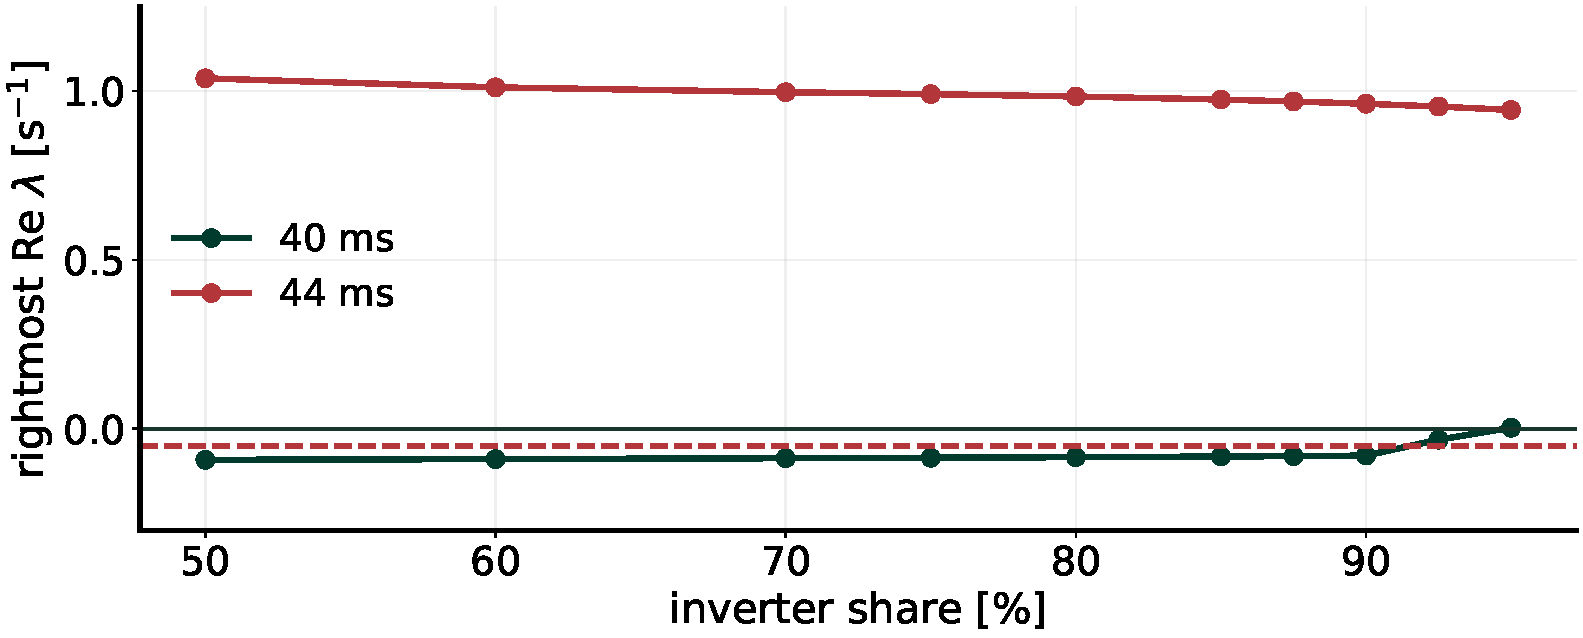
\includegraphics[width=268mm,height=92mm,keepaspectratio]{generated/figures/share_margin.pdf}\par
    {\fontsize{22pt}{25pt}\selectfont Rightmost root versus inverter share (exact delay): at 40 ms the margin holds up to 90\,\% share; at 44 ms the PLL family is unstable at every share from 50\,\%.\par}

  \end{PosterPanel}
\end{minipage}%
